
%% bare_jrnl.tex
%% V1.4
%% 2012/12/27
%% by Michael Shell
%% see http://www.michaelshell.org/
%% for current contact information.
%%
%% This is a skeleton file demonstrating the use of IEEEtran.cls
%% (requires IEEEtran.cls version 1.8 or later) with an IEEE journal paper.
%%
%% Support sites:
%% http://www.michaelshell.org/tex/ieeetran/
%% http://www.ctan.org/tex-archive/macros/latex/contrib/IEEEtran/
%% and
%% http://www.ieee.org/



% *** Authors should verify (and, if needed, correct) their LaTeX system  ***
% *** with the testflow diagnostic prior to trusting their LaTeX platform ***
% *** with production work. IEEE's font choices can trigger bugs that do  ***
% *** not appear when using other class files.                            ***
% The testflow support page is at:
% http://www.michaelshell.org/tex/testflow/


%%*************************************************************************
%% Legal Notice:
%% This code is offered as-is without any warranty either expressed or
%% implied; without even the implied warranty of MERCHANTABILITY or
%% FITNESS FOR A PARTICULAR PURPOSE! 
%% User assumes all risk.
%% In no event shall IEEE or any contributor to this code be liable for
%% any damages or losses, including, but not limited to, incidental,
%% consequential, or any other damages, resulting from the use or misuse
%% of any information contained here.
%%
%% All comments are the opinions of their respective authors and are not
%% necessarily endorsed by the IEEE.
%%
%% This work is distributed under the LaTeX Project Public License (LPPL)
%% ( http://www.latex-project.org/ ) version 1.3, and may be freely used,
%% distributed and modified. A copy of the LPPL, version 1.3, is included
%% in the base LaTeX documentation of all distributions of LaTeX released
%% 2003/12/01 or later.
%% Retain all contribution notices and credits.
%% ** Modified files should be clearly indicated as such, including  **
%% ** renaming them and changing author support contact information. **
%%
%% File list of work: IEEEtran.cls, IEEEtran_HOWTO.pdf, bare_adv.tex,
%%                    bare_conf.tex, bare_jrnl.tex, bare_jrnl_compsoc.tex,
%%                    bare_jrnl_transmag.tex
%%*************************************************************************

% Note that the a4paper option is mainly intended so that authors in
% countries using A4 can easily print to A4 and see how their papers will
% look in print - the typesetting of the document will not typically be
% affected with changes in paper size (but the bottom and side margins will).
% Use the testflow package mentioned above to verify correct handling of
% both paper sizes by the user's LaTeX system.
%
% Also note that the "draftcls" or "draftclsnofoot", not "draft", option
% should be used if it is desired that the figures are to be displayed in
% draft mode.
%
\documentclass[journal]{IEEEtran}
%
% If IEEEtran.cls has not been installed into the LaTeX system files,
% manually specify the path to it like:
% \documentclass[journal]{../sty/IEEEtran}





% Some very useful LaTeX packages include:
% (uncomment the ones you want to load)


% *** MISC UTILITY PACKAGES ***
%
%\usepackage{ifpdf}
% Heiko Oberdiek's ifpdf.sty is very useful if you need conditional
% compilation based on whether the output is pdf or dvi.
% usage:
% \ifpdf
%   % pdf code
% \else
%   % dvi code
% \fi
% The latest version of ifpdf.sty can be obtained from:
% http://www.ctan.org/tex-archive/macros/latex/contrib/oberdiek/
% Also, note that IEEEtran.cls V1.7 and later provides a builtin
% \ifCLASSINFOpdf conditional that works the same way.
% When switching from latex to pdflatex and vice-versa, the compiler may
% have to be run twice to clear warning/error messages.






% *** CITATION PACKAGES ***
%
\usepackage{cite}
% cite.sty was written by Donald Arseneau
% V1.6 and later of IEEEtran pre-defines the format of the cite.sty package
% \cite{} output to follow that of IEEE. Loading the cite package will
% result in citation numbers being automatically sorted and properly
% "compressed/ranged". e.g., [1], [9], [2], [7], [5], [6] without using
% cite.sty will become [1], [2], [5]--[7], [9] using cite.sty. cite.sty's
% \cite will automatically add leading space, if needed. Use cite.sty's
% noadjust option (cite.sty V3.8 and later) if you want to turn this off
% such as if a citation ever needs to be enclosed in parenthesis.
% cite.sty is already installed on most LaTeX systems. Be sure and use
% version 4.0 (2003-05-27) and later if using hyperref.sty. cite.sty does
% not currently provide for hyperlinked citations.
% The latest version can be obtained at:
% http://www.ctan.org/tex-archive/macros/latex/contrib/cite/
% The documentation is contained in the cite.sty file itself.






% *** GRAPHICS RELATED PACKAGES ***
%
\ifCLASSINFOpdf
   \usepackage[pdftex]{graphicx}
  % declare the path(s) where your graphic files are
   \graphicspath{{../pdf/}{../jpeg/}}
  % and their extensions so you won't have to specify these with
  % every instance of \includegraphics
\DeclareGraphicsExtensions{.pdf,.jpeg,.png}
\else
  % or other class option (dvipsone, dvipdf, if not using dvips). graphicx
  % will default to the driver specified in the system graphics.cfg if no
  % driver is specified.
  % \usepackage[dvips]{graphicx}
  % declare the path(s) where your graphic files are
  % \graphicspath{{../eps/}}
  % and their extensions so you won't have to specify these with
  % every instance of \includegraphics
  % \DeclareGraphicsExtensions{.eps}
\fi
% graphicx was written by David Carlisle and Sebastian Rahtz. It is
% required if you want graphics, photos, etc. graphicx.sty is already
% installed on most LaTeX systems. The latest version and documentation
% can be obtained at: 
% http://www.ctan.org/tex-archive/macros/latex/required/graphics/
% Another good source of documentation is "Using Imported Graphics in
% LaTeX2e" by Keith Reckdahl which can be found at:
% http://www.ctan.org/tex-archive/info/epslatex/
%
% latex, and pdflatex in dvi mode, support graphics in encapsulated
% postscript (.eps) format. pdflatex in pdf mode supports graphics
% in .pdf, .jpeg, .png and .mps (metapost) formats. Users should ensure
% that all non-photo figures use a vector format (.eps, .pdf, .mps) and
% not a bitmapped formats (.jpeg, .png). IEEE frowns on bitmapped formats
% which can result in "jaggedy"/blurry rendering of lines and letters as
% well as large increases in file sizes.
%
% You can find documentation about the pdfTeX application at:
% http://www.tug.org/applications/pdftex





% *** MATH PACKAGES ***
%
\usepackage[cmex10]{amsmath}
% A popular package from the American Mathematical Society that provides
% many useful and powerful commands for dealing with mathematics. If using
% it, be sure to load this package with the cmex10 option to ensure that
% only type 1 fonts will utilized at all point sizes. Without this option,
% it is possible that some math symbols, particularly those within
% footnotes, will be rendered in bitmap form which will result in a
% document that can not be IEEE Xplore compliant!
%
% Also, note that the amsmath package sets \interdisplaylinepenalty to 10000
% thus preventing page breaks from occurring within multiline equations. Use:
\interdisplaylinepenalty=2500
% after loading amsmath to restore such page breaks as IEEEtran.cls normally
% does. amsmath.sty is already installed on most LaTeX systems. The latest
% version and documentation can be obtained at:
% http://www.ctan.org/tex-archive/macros/latex/required/amslatex/math/





% *** SPECIALIZED LIST PACKAGES ***
%
%\usepackage{algorithmic}
% algorithmic.sty was written by Peter Williams and Rogerio Brito.
% This package provides an algorithmic environment fo describing algorithms.
% You can use the algorithmic environment in-text or within a figure
% environment to provide for a floating algorithm. Do NOT use the algorithm
% floating environment provided by algorithm.sty (by the same authors) or
% algorithm2e.sty (by Christophe Fiorio) as IEEE does not use dedicated
% algorithm float types and packages that provide these will not provide
% correct IEEE style captions. The latest version and documentation of
% algorithmic.sty can be obtained at:
% http://www.ctan.org/tex-archive/macros/latex/contrib/algorithms/
% There is also a support site at:
% http://algorithms.berlios.de/index.html
% Also of interest may be the (relatively newer and more customizable)
% algorithmicx.sty package by Szasz Janos:
% http://www.ctan.org/tex-archive/macros/latex/contrib/algorithmicx/




% *** ALIGNMENT PACKAGES ***
%
\usepackage{array}
% Frank Mittelbach's and David Carlisle's array.sty patches and improves
% the standard LaTeX2e array and tabular environments to provide better
% appearance and additional user controls. As the default LaTeX2e table
% generation code is lacking to the point of almost being broken with
% respect to the quality of the end results, all users are strongly
% advised to use an enhanced (at the very least that provided by array.sty)
% set of table tools. array.sty is already installed on most systems. The
% latest version and documentation can be obtained at:
% http://www.ctan.org/tex-archive/macros/latex/required/tools/


% IEEEtran contains the IEEEeqnarray family of commands that can be used to
% generate multiline equations as well as matrices, tables, etc., of high
% quality.




% *** SUBFIGURE PACKAGES ***
%\ifCLASSOPTIONcompsoc
%  \usepackage[caption=false,font=normalsize,labelfont=sf,textfont=sf]{subfig}
%\else
%  \usepackage[caption=false,font=footnotesize]{subfig}
%\fi
% subfig.sty, written by Steven Douglas Cochran, is the modern replacement
% for subfigure.sty, the latter of which is no longer maintained and is
% incompatible with some LaTeX packages including fixltx2e. However,
% subfig.sty requires and automatically loads Axel Sommerfeldt's caption.sty
% which will override IEEEtran.cls' handling of captions and this will result
% in non-IEEE style figure/table captions. To prevent this problem, be sure
% and invoke subfig.sty's "caption=false" package option (available since
% subfig.sty version 1.3, 2005/06/28) as this is will preserve IEEEtran.cls
% handling of captions.
% Note that the Computer Society format requires a larger sans serif font
% than the serif footnote size font used in traditional IEEE formatting
% and thus the need to invoke different subfig.sty package options depending
% on whether compsoc mode has been enabled.
%
% The latest version and documentation of subfig.sty can be obtained at:
% http://www.ctan.org/tex-archive/macros/latex/contrib/subfig/




% *** FLOAT PACKAGES ***
%
%\usepackage{fixltx2e}
% fixltx2e, the successor to the earlier fix2col.sty, was written by
% Frank Mittelbach and David Carlisle. This package corrects a few problems
% in the LaTeX2e kernel, the most notable of which is that in current
% LaTeX2e releases, the ordering of single and double column floats is not
% guaranteed to be preserved. Thus, an unpatched LaTeX2e can allow a
% single column figure to be placed prior to an earlier double column
% figure. The latest version and documentation can be found at:
% http://www.ctan.org/tex-archive/macros/latex/base/

\usepackage{threeparttable}

%\usepackage{stfloats}
% stfloats.sty was written by Sigitas Tolusis. This package gives LaTeX2e
% the ability to do double column floats at the bottom of the page as well
% as the top. (e.g., "\begin{figure*}[!b]" is not normally possible in
% LaTeX2e). It also provides a command:
%\fnbelowfloat
% to enable the placement of footnotes below bottom floats (the standard
% LaTeX2e kernel puts them above bottom floats). This is an invasive package
% which rewrites many portions of the LaTeX2e float routines. It may not work
% with other packages that modify the LaTeX2e float routines. The latest
% version and documentation can be obtained at:
% http://www.ctan.org/tex-archive/macros/latex/contrib/sttools/
% Do not use the stfloats baselinefloat ability as IEEE does not allow
% \baselineskip to stretch. Authors submitting work to the IEEE should note
% that IEEE rarely uses double column equations and that authors should try
% to avoid such use. Do not be tempted to use the cuted.sty or midfloat.sty
% packages (also by Sigitas Tolusis) as IEEE does not format its papers in
% such ways.
% Do not attempt to use stfloats with fixltx2e as they are incompatible.
% Instead, use Morten Hogholm'a dblfloatfix which combines the features
% of both fixltx2e and stfloats:
%
% \usepackage{dblfloatfix}
% The latest version can be found at:
% http://www.ctan.org/tex-archive/macros/latex/contrib/dblfloatfix/




%\ifCLASSOPTIONcaptionsoff
%  \usepackage[nomarkers]{endfloat}
% \let\MYoriglatexcaption\caption
% \renewcommand{\caption}[2][\relax]{\MYoriglatexcaption[#2]{#2}}
%\fi
% endfloat.sty was written by James Darrell McCauley, Jeff Goldberg and 
% Axel Sommerfeldt. This package may be useful when used in conjunction with 
% IEEEtran.cls'  captionsoff option. Some IEEE journals/societies require that
% submissions have lists of figures/tables at the end of the paper and that
% figures/tables without any captions are placed on a page by themselves at
% the end of the document. If needed, the draftcls IEEEtran class option or
% \CLASSINPUTbaselinestretch interface can be used to increase the line
% spacing as well. Be sure and use the nomarkers option of endfloat to
% prevent endfloat from "marking" where the figures would have been placed
% in the text. The two hack lines of code above are a slight modification of
% that suggested by in the endfloat docs (section 8.4.1) to ensure that
% the full captions always appear in the list of figures/tables - even if
% the user used the short optional argument of \caption[]{}.
% IEEE papers do not typically make use of \caption[]'s optional argument,
% so this should not be an issue. A similar trick can be used to disable
% captions of packages such as subfig.sty that lack options to turn off
% the subcaptions:
% For subfig.sty:
% \let\MYorigsubfloat\subfloat
% \renewcommand{\subfloat}[2][\relax]{\MYorigsubfloat[]{#2}}
% However, the above trick will not work if both optional arguments of
% the \subfloat command are used. Furthermore, there needs to be a
% description of each subfigure *somewhere* and endfloat does not add
% subfigure captions to its list of figures. Thus, the best approach is to
% avoid the use of subfigure captions (many IEEE journals avoid them anyway)
% and instead reference/explain all the subfigures within the main caption.
% The latest version of endfloat.sty and its documentation can obtained at:
% http://www.ctan.org/tex-archive/macros/latex/contrib/endfloat/
%
% The IEEEtran \ifCLASSOPTIONcaptionsoff conditional can also be used
% later in the document, say, to conditionally put the References on a 
% page by themselves.




% *** PDF, URL AND HYPERLINK PACKAGES ***
%
%\usepackage{url}
% url.sty was written by Donald Arseneau. It provides better support for
% handling and breaking URLs. url.sty is already installed on most LaTeX
% systems. The latest version and documentation can be obtained at:
% http://www.ctan.org/tex-archive/macros/latex/contrib/url/
% Basically, \url{my_url_here}.




% *** Do not adjust lengths that control margins, column widths, etc. ***
% *** Do not use packages that alter fonts (such as pslatex).         ***
% There should be no need to do such things with IEEEtran.cls V1.6 and later.
% (Unless specifically asked to do so by the journal or conference you plan
% to submit to, of course. )


% correct bad hyphenation here
\hyphenation{op-tical net-works semi-conduc-tor}


\begin{document}
%
% paper title
% can use linebreaks \\ within to get better formatting as desired
% Do not put math or special symbols in the title.
\title{Heartbeats Classification Using Autoencoder-Based Deep Network with Massive Electrocardiography}
%
%
% author names and IEEE memberships
% note positions of commas and nonbreaking spaces ( ~ ) LaTeX will not break
% a structure at a ~ so this keeps an author's name from being broken across
% two lines.
% use \thanks{} to gain access to the first footnote area
% a separate \thanks must be used for each paragraph as LaTeX2e's \thanks
% was not built to handle multiple paragraphs
%

\author{Yan~Yan,~
        Xingbin~Qin,~
        Jianping~Fan,~
        and~Lei~Wang~% <-this % stops a space
\thanks{Y. Yan is with the Shenzhen Key Laboratory for Low-cost Healthcare, Shenzhen Institutes of Advanced Technology, Chinese Academy of Sciences. No. 1068, Xueyuan Road, Nanshan District,
Shenzhen, Guangdong Province, China-mail: (yan.yan@siat.ac.cn).}% <-this % stops a space
\thanks{X. Qin is with the Shenzhen Institutes of Advanced Technology, Chinese Academy of Sciences.
No. 1068, Xueyuan Road, Nanshan District, Shenzhen, Guangdong Province, China.}% <-this % stops a space
\thanks{J. Fan is with the Shenzhen Institutes of Advanced Technology, Chinese Academy of Sciences. No. 1068, Xueyuan Road, Nanshan District, Shenzhen, Guangdong Province, China.}% <-this % stops a space
\thanks{L. Wang is with the Shenzhen Key Laboratory for Low-cost Healthcare, Shenzhen Institutes of Advanced Technology, Chinese Academy of Sciences.
No. 1068, Xueyuan Road, Nanshan District,
Shenzhen, Guangdong Province, China.}% <-this % stops a space
\thanks{Manuscript received September 29, 2014; revised}}

% note the % following the last \IEEEmembership and also \thanks - 
% these prevent an unwanted space from occurring between the last author name
% and the end of the author line. i.e., if you had this:
% 
% \author{....lastname \thanks{...} \thanks{...} }
%                     ^------------^------------^----Do not want these spaces!
%
% a space would be appended to the last name and could cause every name on that
% line to be shifted left slightly. This is one of those "LaTeX things". For
% instance, "\textbf{A} \textbf{B}" will typeset as "A B" not "AB". To get
% "AB" then you have to do: "\textbf{A}\textbf{B}"
% \thanks is no different in this regard, so shield the last } of each \thanks
% that ends a line with a % and do not let a space in before the next \thanks.
% Spaces after \IEEEmembership other than the last one are OK (and needed) as
% you are supposed to have spaces between the names. For what it is worth,
% this is a minor point as most people would not even notice if the said evil
% space somehow managed to creep in.



% The paper headers
\markboth{Journal of Biomedical and Health Informatics,~Vol.~, No.~, September~2014}%
{Shell \MakeLowercase{\textit{et al.}}: Bare Demo of IEEEtran.cls for Journals}
% The only time the second header will appear is for the odd numbered pages
% after the title page when using the twoside option.
% 
% *** Note that you probably will NOT want to include the author's ***
% *** name in the headers of peer review papers.                   ***
% You can use \ifCLASSOPTIONpeerreview for conditional compilation here if
% you desire.




% If you want to put a publisher's ID mark on the page you can do it like
% this:
%\IEEEpubid{0000--0000/00\$00.00~\copyright~2012 IEEE}
% Remember, if you use this you must call \IEEEpubidadjcol in the second
% column for its text to clear the IEEEpubid mark.



% use for special paper notices
%\IEEEspecialpapernotice{(Invited Paper)}




% make the title area
\maketitle

% As a general rule, do not put math, special symbols or citations
% in the abstract or keywords.
\begin{abstract}
A Big Data approach for the classification of heartbeat in electrocardiography analysis is presented. Based on massive heartbeat wave samples extracted from ambulatory ECG dataset, a deep neural network structure with a stacked autoencoder pretraining with fine-tuning algorithm is adopted for classification of normal heartbeat, supraventricular ectopic heartbeat, ventricular ectopic heartbeat, fusion heartbeat based on the ANSI/AAMI EC57: 1998/(R)2008 standard. The MIT-BIH arrhythmia database and MIT-BIH long term ECG database are also involved in the database, with the unlabelled database they were divided into three datasets for unsupervised pretraining, supervised fine-tuning and test. From the massive unlabelled dataset, representations learned from the raw sample were acquired by the training algorithm and structure. A significant improvement from the reported results for heartbeat classification is attained for the classification task with the parameters: accuracy to $99.34\%$, normal heartbeat specificity $99.76\%$, supraventricular ectopic heartbeat sensitivity $82.29\%$, ventricular ectopic heartbeat sensitivity $98.31\%$ and fusion heartbeat sensitivity $87.71\%$. The proposed method might be generalized to other related applications with large amount of unlabelled data from the long-term clinical monitoring and healthcare monitoring. 


\end{abstract}

% Note that keywords are not normally used for peerreview papers.
\begin{IEEEkeywords}
big data, electrocardiography classification, sparse autoencoder, deep learning.
\end{IEEEkeywords}






% For peer review papers, you can put extra information on the cover
% page as needed:
 \ifCLASSOPTIONpeerreview
 \begin{center} \bfseries EDICS Category: 3-BBND \end{center}
 \fi
%
% For peerreview papers, this IEEEtran command inserts a page break and
% creates the second title. It will be ignored for other modes.
\IEEEpeerreviewmaketitle



\section{Introduction}
% The very first letter is a 2 line initial drop letter followed
% by the rest of the first word in caps.
% 
% form to use if the first word consists of a single letter:
% \IEEEPARstart{A}{demo} file is ....
% 
% form to use if you need the single drop letter followed by
% normal text (unknown if ever used by IEEE):
% \IEEEPARstart{A}{}demo file is ....
% 
% Some journals put the first two words in caps:
% \IEEEPARstart{T}{his demo} file is ....
% 
% Here we have the typical use of a "T" for an initial drop letter
% and "HIS" in caps to complete the first word.
\IEEEPARstart{A}{n} era of big data in healthcare is now under way, decades of progress in digitising medical records accumulate vast amounts of medical data, simultaneously mobile healthcare and wearable sensor technologies offer healthcare data from larger population coverage.
The noninvasive, inexpensive and well-established technology of electrocardiographic signal in mobile health or personal health has the greatest popularity in heart function analysis.
Automated electrocardiography classification provides indispensable assist in long-term clinical monitoring, and a large number of approaches have been proposed for the task, easing the diagnosis of arrhythmic changes as well as further inspection, e.g., heart rate variability or heart turbulence analysis \cite{mar}. 


Lots of algorithms have been proposed for the classification and detection for electrocardiography signals. 
The electrocardiography classification or detection task had been divided into two parts: the feature extraction process and classifier. 
Simple classifier such as linear discriminants \cite{chaza} and kNN \cite{melgan}, more complex classifiers like neural networks \cite{jiang, olmez, lin, osowski}, fuzzy inference engines \cite{osowski, kundu}, hidden Markov model \cite{andreao, coast}, independent component analysis \cite{zhu} and support vector machine  \cite{melgan, kampoura, khandoker} were also adapted by lots of researchers.  

 
Beyond the classifier, the performance of a recognition system highly depends on the determination of extracted electrocardiography features. Time domain features, frequency domain features, and statistical measures features for six fundamental waves (PQRSTU) had been used in feature extraction process \cite{chia}. 
Time domain features like morphological features include shapes, amplitudes, and durations were adapted primarily in \cite{jekova, christove, can}, frequency domain features like wavelet transformation were widely used \cite{inan}, \cite{banerjee} stationary features like higher order statistics also had been developed. 
Principal component analysis \cite{stam} and Hermite functions \cite{lager} have been used in electrocardiography classification and related analysis technologies as well.
Almost every single published paper proposes a new set of features to be used, or a new combination of the existing ones \cite{mar}.


The results from these algorithms or models were not amenable to expert labelling, as well as for the identification of complex relationships between subjects and clinical conditions \cite{clifford}.
But for the ambulatory electrocardiography clinical application, as well as the normal application in daily healthcare monitoring for cardiac function or early warning of heart disease, an automated algorithm or model would have significant meaning.
The application of artificial intelligence methods has become an important trend in electrocardiography for the recognition and classification of different arrhythmia types \cite{clifford}. 
The data explosion puts forward the new request to the method of data processing and information mining.


Over the past decades computational techniques proliferated in the pattern recognition field, simultaneously the applications in electrocardiography recognition, detection and classification for relevant trends, patterns, and outliers. 
Most of the literatures in the electrocardiography classification task were focused on the supervised learning methods, as in unsupervised learning methods were infrequently used, which needs a lot of effort in labelling data. The MIT-BIH database \cite{physionet} was the most widely used data in the classification and detection algorithm developments, while mass unlabelled electrocardiography data had been ignored due to the supervise learning approaches essential. 
Unsupervised learning methods become crucial in mining or analysing unlabelled data, as the unlabelled electrocardiography data accumulated. Unsupervised learning-based approaches and the application to electrocardiogram classification in literatures mainly include clustering-based techniques \cite{lager, nishizawa, maier}, self-adaptive neural network-based methods \cite{palreddy, risk} and some hybrid unsupervised learning systems \cite{tadejko}. 

In this paper, we adopt a big data unsupervised learning approach of sparse autoencoder based deep neural network in large unlabelled ambulatory electrocardiography dataset to learn features automatically, with which the cardiac arrhythmia with electrocardiograms classification task was proposed. 

In the following sections, we will first state the experimental setup and methodologies in Section 2. Then the experimental results and the discussion are given in Section 3 and Section 4 respectively.

\section{Electrocardiography Datasets and Arrhythmia Classes}



\begin{table*}[!htbp]
\begin{center}
\begin{threeparttable}
\caption{AAMI Classes Mapped from MIT-BIH Arrhythmia \& Long-term Database Types}
\label{Table1}
\begin{tabular}{cllllll}
\hline
& AAMI heartbeat classes & N & S & V & F & Q \\
& Description  &Any heartbeat not in & Supraventricular ectopic  & Ventricular ectopic  & Fusion beat & Unknown beat \\
&                     &the S,V,F or Q class & beat   		     & beat	      &	     &          \\
\hline
& MIT-BIH heartbeat  &Normal beat (1)            & Aberrated atrial premature & Ventricular escape & Fusion of ventricular& Paced beat (12)\\
&  types (codes)   &  					  &  beat (11)		    &  beat(10)	            & \& normal beat (6)		      &             \\

&                     &Left bundle branch   &  Nodal (junctional) &Premature ventricular& 	 &  Unclassifiable \\
&                     &block beat (2)            & premature beat (7)    &contraction (5)         &	   & beat (13)   \\

&                     & Right bundle branch & Atrial premature & Ventricular flutter &    &  Fusion of paced  \\
&                     & block beat (3) & contraction (8)     & wave (31) & 	   & and normal (38)  \\

&                     & Nodal escape  & Premature or ectopic & 	     &  &                          \\
&                     & beat (11)	  & supraventricular beat(9) &     &   &     \\

&                     & Atrial escape beat (34)   &  	  				      & 				            & 			      &                          \\
\hline
& MITBIH-AR$^a$(100,687) & 89,925$^b$   & 2,774   & 7,171   & 802    & 15        \\
& MITBIH-LT(667,347) & 600,197  &  150  & 64,090  & 	2,906   & 0       \\

\hline
\end{tabular}
\begin{tablenotes}
\item [a] Recording 102, 104, 107, 217 were removed.
\item [b] The counts listed in the table may differ from other literatures \cite{chaza} due to the computation need.
\end{tablenotes}
\end{threeparttable}

\end{center}
     \end{table*}





In the proposed method for electrocardiography classification, the unlabelled dataset and labelled datasets are both used. In this section, a general description of the unlabelled pretraining dataset is proposed, then the arrhythmia classification classes used in the labelled open datasets were discussed.



\subsection{Arrhythmia Classes}
The related experiments in this paper were carried out in two public databased available on Physionet, and a collected unlabelled ambulatory electrocardiography database (unlabelled means there were no electrocardiography experts involved in the interpretation). 
The ANSI/AAMI EC57: 1998/(R)2008 standard AAMI (2008) recommends to group the heartbeats into five classes: on-ectopic beats (N); supraventricular ectopic beat (S); ventricular ectopic beat (V); fusion of a V and a N (F); unknown beat type (Q).
As Table \ref{Table1} illustrated the detail of the MIT-BIH Arrhythmia Database and MIT-BIH Long-term Database which mapped to the AAMI heartbeat classes.


\subsection{The Unlabelled Dataset}
Data from the ambulatory electrocardiography database were used in this study, which includes recordings of 100 subjects with arrhythmia along with normal sinus rhythm. The database contains 100 recordings, each containing a 3-lead 24-hour long electrocardiography which were bandpass filtered at 0.1-100Hz and sampled at 128Hz. In this study, only the lead \uppercase\expandafter{\romannumeral1} data were adapted after preprocessing in the classification task. The reference average heart beats for each sample has 97,855 beats for the 24-hour long recording, and the reference arrhythmia average is 1,810 beats which were estimated by a commercial software (this statistics aim to indicate the existence for arrhythmia samples, which should not be consider as a experiment preset).

\subsection{The Open Labelled Datasets}
The MIT-BIH Arrhythmia Database \cite{physionet} contains 48 half-hour recordings each containing two 30-min ECG lead signals (lead A and lead B), sampled at 360Hz. As well only the  lead \uppercase\expandafter{\romannumeral1} data were used in the proposed method. In agreement with the AAMI recommended practice, the four recordings with paced beats were removed from the analysis. The remaining recordings were divided into two datasets, with small part of which were used as the training set of the fine-tuning process (details would be described in the following part).
The MIT-BIT Long-term Database is also used in this study for training and verification, which contains 7 long-term ECG recordings (14 to 22 hours each), with manually reviewed beat annotations and sampled at 128Hz. Similarly, the 7 recordings were divided into two datasets, with part used as the fine-tuning training set. A description of the labelled datasets are illustrated in Table \ref{Table1}.



\section{Experimental Methodology}
In this section, the proposed approach technic details are described. This section includes descriptions of the deep architectures, the auto-encoder based training method, the data sets used, the classification task settings and other necessary details.
\subsection{Models}
Deep learning methods attempt to learn feature hierarchies as higher-level features are formed by the composition of lower-level features. The electrocardiography interpretation has been judged by the medical professionals, which was based on the abstractions of the perceptible features. In this model we consider the higher-level abstractions as the perceptible features, with whose composition the medical professionals can make arrhythmia judgement. The deep architecture automatic learning method is especially important for high-level abstractions, which human often do not know how to specify explicitly in terms of raw sensory input \cite{erhan}. As \cite{collobert} discussed, deep learning methods are bused on learning internal representations of data, another important advantage they offer is the ability to naturally leverage: (a) unsupervised data and (b) data from similar tasks to boost performance on large and challenging problems that routinely suffer from a poverty of labelled data. In the electrocardiography classification problem, we got plenty of unsupervised data, and the labelled data was limited as well, so it is a spontaneously idea to adapt deep learning method in this classification problem.


\subsubsection{Deep Neural Networks}
The artificial neural network had been widely used in different applications, the basic 3-layer model (with only one hidden layer) is a fairly shallow network which means only shallow features can be learning via the structure. Deep neural networks, meaning ones in which we have multiple hidden layers, with which we can compute much more complex features of the input. Each hidden layer computes a non-linear transformation of the previous layer, a deep network can have significantly greater representational power (i.e., can learn significantly more complex functions) than a shallow one. A typical deep neural network structure makes no different from the normal multi layer neural network.




\subsubsection{Autoencoders and Sparsity}
\begin{figure}[]
\centering
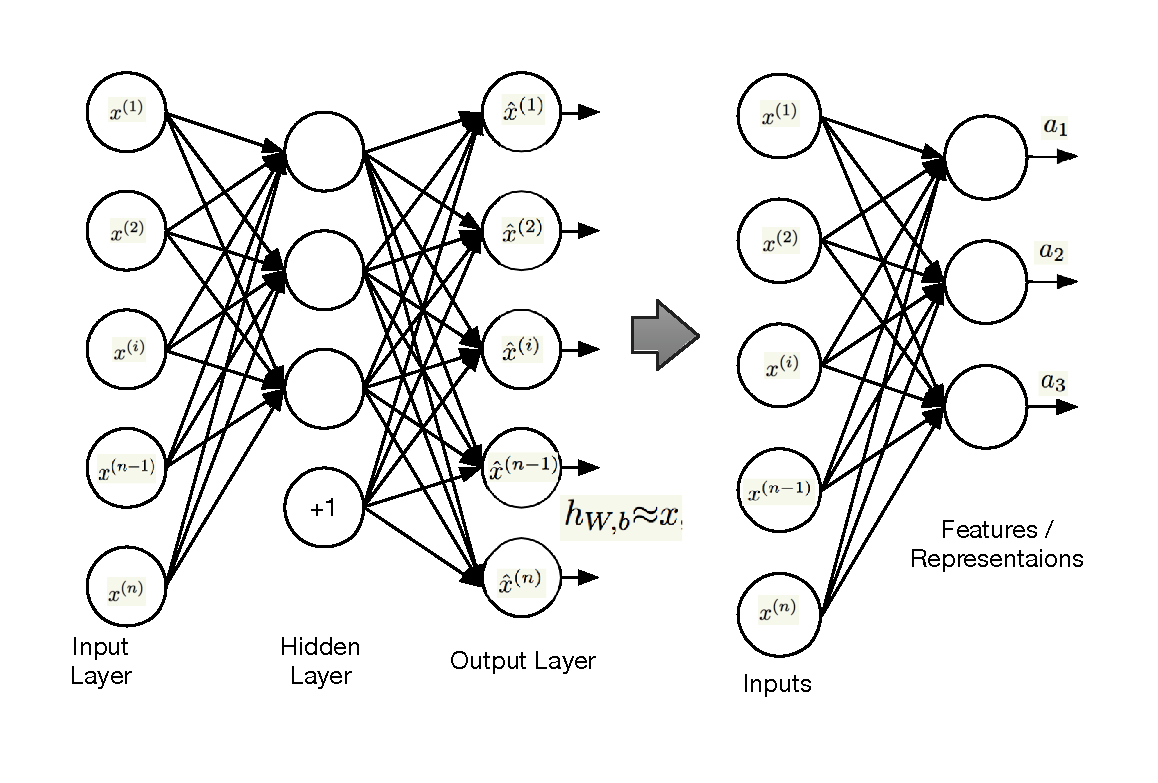
\includegraphics[width=3.2 in]{Figure1}
% where an .eps filename suffix will be assumed under latex, 
% and a .pdf suffix will be assumed for pdflatex; or what has been declared
% via \DeclareGraphicsExtensions.
\caption{An one-hidden-layer autoencoder: first preset the output of the autoencoder to be the same as itself, train the neural network, then use the learned weights of the connections to calculate the representations of the raw input, in some literatures the process could be encoder and decoder \cite{bengio2009}.}
\label{figure1}
\end{figure}

An autoencoder is trained to encode the input $x$ into some representation $c(x)$ so that the input can be reconstructed from that representation \cite{bengio2009}. 
The autoencoder neural network is an unsupervised learning algorithm that applies backpropagation, setting the target values to be equal to the inputs. i.e it uses $y^{(i)}=x^{(i)}$. The autoencoder neural network illustrated in Fig2 tries to learn a function $h_{W,b}{\approx}x$, which tries to approach a identity function to ensure the output $\hat{x_1}$ close to $x$. If there is one linear hidden layer and the mean squared error criterion is used to train the network, then the k hidden units learn to project the input in the span of the first $k$ principal components of the data \cite{bourlard}. Since in the neural network the hidden layer is nonlinear, the autoencoder behaves differently from PCA, which has the ability to capture multi-modal aspects of the input distribution (the representation of the input) \cite{jap}. The related literature experiments reported in \cite{bengio2007} suggest that in practice, when trained with stochastic gradient descent, nonlinear autoencoders with more hidden units than inputs (called overcomplete) yield useful representations (in the sense of classification error measured on a network taking this representation in input). A farther defence of autoencoder can be accessed from \cite{bengio2009}.
As the theory illustrated, the electrocardiography signal representations can be learned via the autoencoder structures and algorithms. 

In the adapted algorithm, we impose a sparsity constraint on the hidden units to guarantee the representations expression ability.
The neuron would be considered as ``active" or ``firing" if its output value by the activation function is close to $1$, or as being ``inactive" if its output value is close to $0$ in which the $sigmoid$ activation function adapted. The correspond numerical value would be $1$ and $-1$ with $tanh$ activation function. $a_j^{(2)}(x)$ denote the activation of hidden unit $j$ in the autoencoder with the given input of $x$. 
And farther, let 

\begin{equation}
\hat{\rho}_j = \frac{1}{m} \sum_{i=1}^m [{a_j^{(2)}}{(x^{(i)})}]
\end{equation}

\noindent be the average activation of hidden unit $j$ (averaged over the training set). Approximately enforce the constraint:

\begin{equation}
\hat{\rho}_j = \rho
\end{equation}

where $\rho$ is a sparsity parameter, typically a small value close to zero (such as $\rho = 0.05$), which means the average activation of each hidden neuron $j$ to be close to zero (0.05 for instance). 

The overall cost function of neural network is denoted by $J(W,b)$ which was defined by:

\begin{equation}
\begin{split}
J(W,b) = [\frac{1}{m}\sum_{i=1}^m(\frac{1}{2}{\|{h_{W,b}(x^{(i)})} - y^{(i)}\|}^2)] \\
+ \frac{\lambda}{2}\sum_{l=1}^{n_l-1} \sum_{i=1}^{s_l} \sum_{j=1}^{s_l+1}{W_{ji}^{(l)}}^2
\end{split}
\end{equation}

\noindent as the first term in the definition of $J(W,b)$ is an average sum-of-squares error term. The second term is a regularization term that tends to decrease the magnitude of the weights, and helps prevent overfitting. The definition of $\lambda$, $s$, $l$ etc. would be explained in detail in the appendix part. To satisfy the constraint of sparsity, an extra penalty term to the optimisation objective that penalised $\hat{\rho}_j $ deviating significantly from $\rho$. The Kullback-Leibler (KL) divergence:

\begin{equation}
 \sum_{j=1}^{s_2}KL(\rho||\hat{\rho}) =  \sum_{j=1}^{s_2}\rho \text{log}{\frac{\rho}{\hat{\rho}_j}}+(1-\rho)\text{log}\frac{1-\rho}{1-\hat{{\rho}_j}}
\end{equation}

\noindent is chosen as the  penalty term. KL-divergence is a standard function for measuring how different two different distributions are. So in the autoencoder neural network training, the cost function of $J_{sparse}(W,b)$ was defined as:

\begin{equation}
J_{sparse}(W,b) = J(W,b) + \beta \sum_{j=1}^{s_2}KL(\rho||\hat{\rho_j})
\end{equation}
\noindent $\beta$ denotes the weight of the sparsity penalty term.

\subsubsection{Feature Self-taught Learning}
The mechanism of how the autoencoder neural network has been used to learn features from unlabelled data had been illustrated in the above sections. Concretely, the collected unlabelled data training set $\{{x_u^{(1)}, x_u^{(2)}, x_u^{(3)}, \ldots, x_u^{(m_u)} }\}$ in which $u$ for the unlabelled. The unlabelled data then had been used in the autoencoder training process. Then the activation $a$ would be calculated by the model parameters of $W^{(1)}$, $b^{(1)}$, $W^{(2)}$, $b^{(2)}$ in the autoencoder illustrated in Fig 2, which would be considered as a better representation (or feature) than the raw input $x$. As well we can adapt the same method in the limited supervised dataset $\{(x_l^{(1)}, y^{(1)}), (x_l^{(2)}, y^{(2)}), \ldots, (x_l^{(m_l)}, y^{(m_l)})\}$,  the supervised dataset has been represented in $\{(a_l^{(1)}, y^{(1)})$, $(a_l^{(2)}, y^{(2)}), \ldots, (a_l^{(m_l)}, y^{(m_l)}) \}$. Finally, after the transformation, a supervised learning algorithm (SVM, logistic regression, Softmax, etc.) could be used for classification tasks. 

\subsubsection{Training Stacked Autoencoders}
Autoencoders have been used as building blocks to build and initialize a deep multi-layer neural network. The training procedure would be \cite{bengio2009}:
\begin{enumerate}
\item Train the first layer as an autoencoder to minimise some form for reconstruction error of the raw input. This is unsupervised.
\item The hidden units' outputs of the autoencoder are now used as input for another layer, also trained to be an autoencoder. Here unlabelled representations were used as well.
\item Iterates as in 2) to initialize the desired number of additional layers.
\item Take the last hidden layer output as input to a supervised layer and initialize its parameters (either randomly or by supervised training, keeping the rest of the network fixed).
\item Fine tune all the parameters of this deep architecture with respect to the supervised criterion. Alternately, unfold all the autoencoders into a very deep autoencoder and fine-tune the global reconstruction error.
\end{enumerate}

The greedy layer-wise approach for pretraining a deep network works by training each layer in turn as explained in step 2). Assume $a^{(n)}$ as the deepest activation of the autoencoder network, then $a^{(n)}$ is a higher level representation than any lower layers, which contains what we interested in. Then the higher level representations (the corresponding features in the traditional artificial selected features) can be used as the classifier input.

\subsubsection{Fine-tuning}
For the training method of stacked autoencoders, when the parameters of one layer are being trained, parameters in other layer are kept fixed. In order to achieve better result, fine-tuning using backpropagation can be used to improve the model performance by tuning the parameters of all layers are changed at the same time after the layer-wise train phase.

\subsubsection{Softmax Classifier}
The cardiac arrhythmia classification problem is a kind of classification problems where the class label $y$ may take more than two possible values (the setting of the classes about the classification would be discussed in the following sections). Softmax regression is a supervised learning algorithm which would be adapted as the classifier in conduction with our proposed deep learning (unsupervised) feature (representation) learning methods. 

Softmax regression model was generalized  from the logistic regression. Similar to the logistic regression, the training set

\begin{equation}
\{(x^{(1)},y^{(1)}), (x^{(2)},y^{(2)}), \ldots, (x^{(m)},y^{(m)}) \}
\end{equation}

\noindent of m labelled examples, the input features are $x^{(i)} \in \Re^{(n+1)}$ (with $x_0$ corresponding to there intercept term). The labels are denoted by 

\begin{equation}
y^{(i)} \in \{1,2,3,\ldots,k\}
\end{equation}
\noindent which means $k$ classes.
Given a test input $x$, the hypothesis to estimate the probability that $p(y=j|x)$ for each value of $j=1,\ldots,k$. I.e., the probabilities of the class labels taking on the $k$ different possible values are estimated. 

\begin{equation}
h_{\theta}(x^{(i)}) = 
\left[
      \begin{array}{cccccc}
        p(y^{(i)}=1|x^{(i)};\theta) \\
        p(y^{(i)}=2|x^{(i)};\theta) \\
        \vdots \\
        p(y^{(i)}=k|x^{(i)};\theta)
      \end{array}
    \right]
\end{equation}
\begin{equation}
= \frac{1}{\sum_{j=1}^ke^{\theta_j^Tx^{(i)}}}
\left[
      \begin{array}{cccccc}
        e^{\theta_1^Tx^{(i)}}\\
        e^{\theta_2^Tx^{(i)}}\\
        \vdots \\
        e^{\theta_k^Tx^{(i)}}
      \end{array}
    \right]
\end{equation}
\noindent in which $\theta_1,\theta_2,\ldots,\theta_k \in \Re^{(n+1)}$ are parameters of the model. The term $\frac{1}{\sum_{j=1}^ke^{\theta_j^Tx^{(i)}}}$ was normalizes the distribution, so that it sums to one.
The cost function adopted for softmax regression is:

\begin{equation}
J(\theta) = -\frac{1}{m}[\sum_{i=1}^m\sum_{j=1}^k1\{y^{(i)}=j\}\text{log}{\frac{e^{\theta_j^Tx^{(i)}}}{\sum_{l=1}^ke^{\theta_l^Tx^{(i)}}}}]
\end{equation}

where $1\{\cdot\}$ is the indicator function. There is no known closed-form way to solve for the minimum of $J(\theta)$, and an iterative optimisation algorithm synch as gradient descent of L-BFGS could be used for the minimal value.
Taking derivatives, the gradient would be:
\begin{equation}
\bigtriangledown_{\theta_j}J(\theta) = -\frac{1}{m}\sum_{i=1}^m[x^{(i)}(1\{y^{(i)}=j\}-p(y^{(i)}=j|x^{(i)};\theta))]
\end{equation}
With this formula for the derivative plugged into an algorithm such as gradient descent, the minimal of $J(\theta)$ could be achieved. The iteration equation of:

\begin{equation}
\theta_j :=\theta_j - \alpha{\bigtriangledown_{\theta_j}J(\theta)}   (\text{for each} j = 1,\ldots,k)
\end{equation}

Generally, the weight decay:
\begin{equation}
\frac{\lambda}{2} \sum_{i=1}^k \sum_{j=0}^n \theta_{jk}^2 (\lambda>0)
\end{equation}
would be incorporated as well, with which the cost function $J(\theta)$ would be strictly convex and a unique solution would be guaranteed. The Hessian is now invertible, and because $J(θ)$ is convex, algorithms such as gradient descent, L-BFGS, etc. are guaranteed to converge to the global minimum.
So the cost function and iteration equations would be:

\begin{equation}
\begin{split}
J(\theta) = -\frac{1}{m}[\sum_{i=1}^m\sum_{j=1}^k1\{y^{(i)}=j\}\text{log}{\frac{e^{\theta_j^Tx^{(i)}}}{\sum_{l=1}^ke^{\theta_l^Tx^{(i)}}}}] \\
+ \frac{\lambda}{2} \sum_{i=1}^k \sum_{j=0}^n \theta_{jk}^2 (\lambda>0)
\end{split}
\end{equation}

and

\begin{equation}
\begin{split}
\bigtriangledown_{\theta_j}J(\theta) = -\frac{1}{m}\sum_{i=1}^m[x^{(i)}(1\{y^{(i)}=j\}-p(y^{(i)}=j|x^{(i)};\theta))] \\
+ \lambda\theta_j  (\lambda>0)
\end{split}
\end{equation}
By minimising $J(\theta)$ with respect to $\theta$, the softmax regression classifier would work properly for the classification task.

\subsection{Setup and Workflow}
Similar to the routine of electrocardiography classification task, the workflow consists of three stages: a prepossessing stage, a processing stage, and a classification stage. The prepossessing stage related technologies are not the focus of this study, so the classical methods for prepossessing were adapted and just a brief introduction of the details would be mentioned. The processing stage and classification stage related theories and technologies had been illustrated in last section. 

\subsubsection{ECG Filtering}
In the preprocessing stage, filtering algorithms were adapted to remove the artefact signals from the ECG signal. The signals include baseline wander, power line interference, and high-frequency noise. In the traditional ECG classification tasks, the filtering process may affect the results more or less, but in this study, the proposed autoencoder networks structure has the characteristics to predict the missing values from the non-missing values \cite{bengio2009}, which means even the input signal might be distorted corrupted by the noise interference, the autoencoder has the ability to undo the effect of a corruption process stochastically applied to the input of the autoencoder, a farther description of the essentials is in \cite{vincent}, and in the results section a contrast would be proposed. For the unlabelled database of ambulatory ECG and the MITBIH LT database, the Lead \uppercase\expandafter{\romannumeral1} data were extracted and a resample from 128Hz to 360Hz procedure was adopted for data consistency.

\subsubsection{Heartbeat Detection}
For the heartbeat detection, the MIT-BIH database and unlabelled database, the positions of R waves are determined. The provided fiducial points of R wave had been used as the basis of wave segmentation. The details of the implementation of R wave detection would not be described in this study, and a reference for the R wave detection algorithms had been explored in \cite{afonso}.

\subsubsection{Heartbeat Segementation}
In the heartbeat segmentation process, the segmentation program of Laguna et al.\footnote{``ecgpuwave", check the website of Physionet} was adapted, which also had been validated by other related work \cite{chaza}. The segmentation process was focus on the  Lead \uppercase\expandafter{\romannumeral1} of the recordings. After the segmentation for the ambulatory ECG database, three batches of heartbeat samples listed in Table \ref{table2} were acquired for the classification task. As for the pretraining, fine-tuning for our proposed task and comparison, we divided all the samples into three groups: the pretraining group as DS1, the fine-tuning group as DS2 and test group as DS3 (illustrated in Table \ref{table3}). Samples are chosen randomly from the original AR and LT database, the details of the sample class would be described in the experiment result analysis.

\begin{table}[!htbp]
\begin{center}
\begin{threeparttable}
\caption{Samples after Segementation}

\label{table2}
\begin{tabular}{cccc}
\hline
& Ambulatory ECG Database (AECG) & MITBIH-AR &  MITBIH-LT\\
\hline
& 9,785,500 & 100,687 &  667,343 \\
\hline
\end{tabular}

\end{threeparttable}

\end{center}
     \end{table}
     
     \begin{table}[!htbp]
\begin{center}
\begin{threeparttable}
\caption{Samples Dataset Settings}
\label{table3}
\begin{tabular}{ccccc}
\hline
& Dataset & DS1& DS2 &  DS3\\
\hline
& Useage & Pretraining & Fine-tuning & Test \\
\hline
& Source (samples) & AECG (9,785,500)   &  &   \\
&  & AR (50,193) & AR (33,663) & AR (16,831) \\
& & LT (587,347)& LT (50,000) & LT (30,000) \\
\hline
&Total & 10,423,040 & 83,633 & 46,831 \\
\hline
\end{tabular}
\end{threeparttable}
\end{center}
\end{table}

\subsubsection{Pretraining}

\begin{figure*}[]
\centering
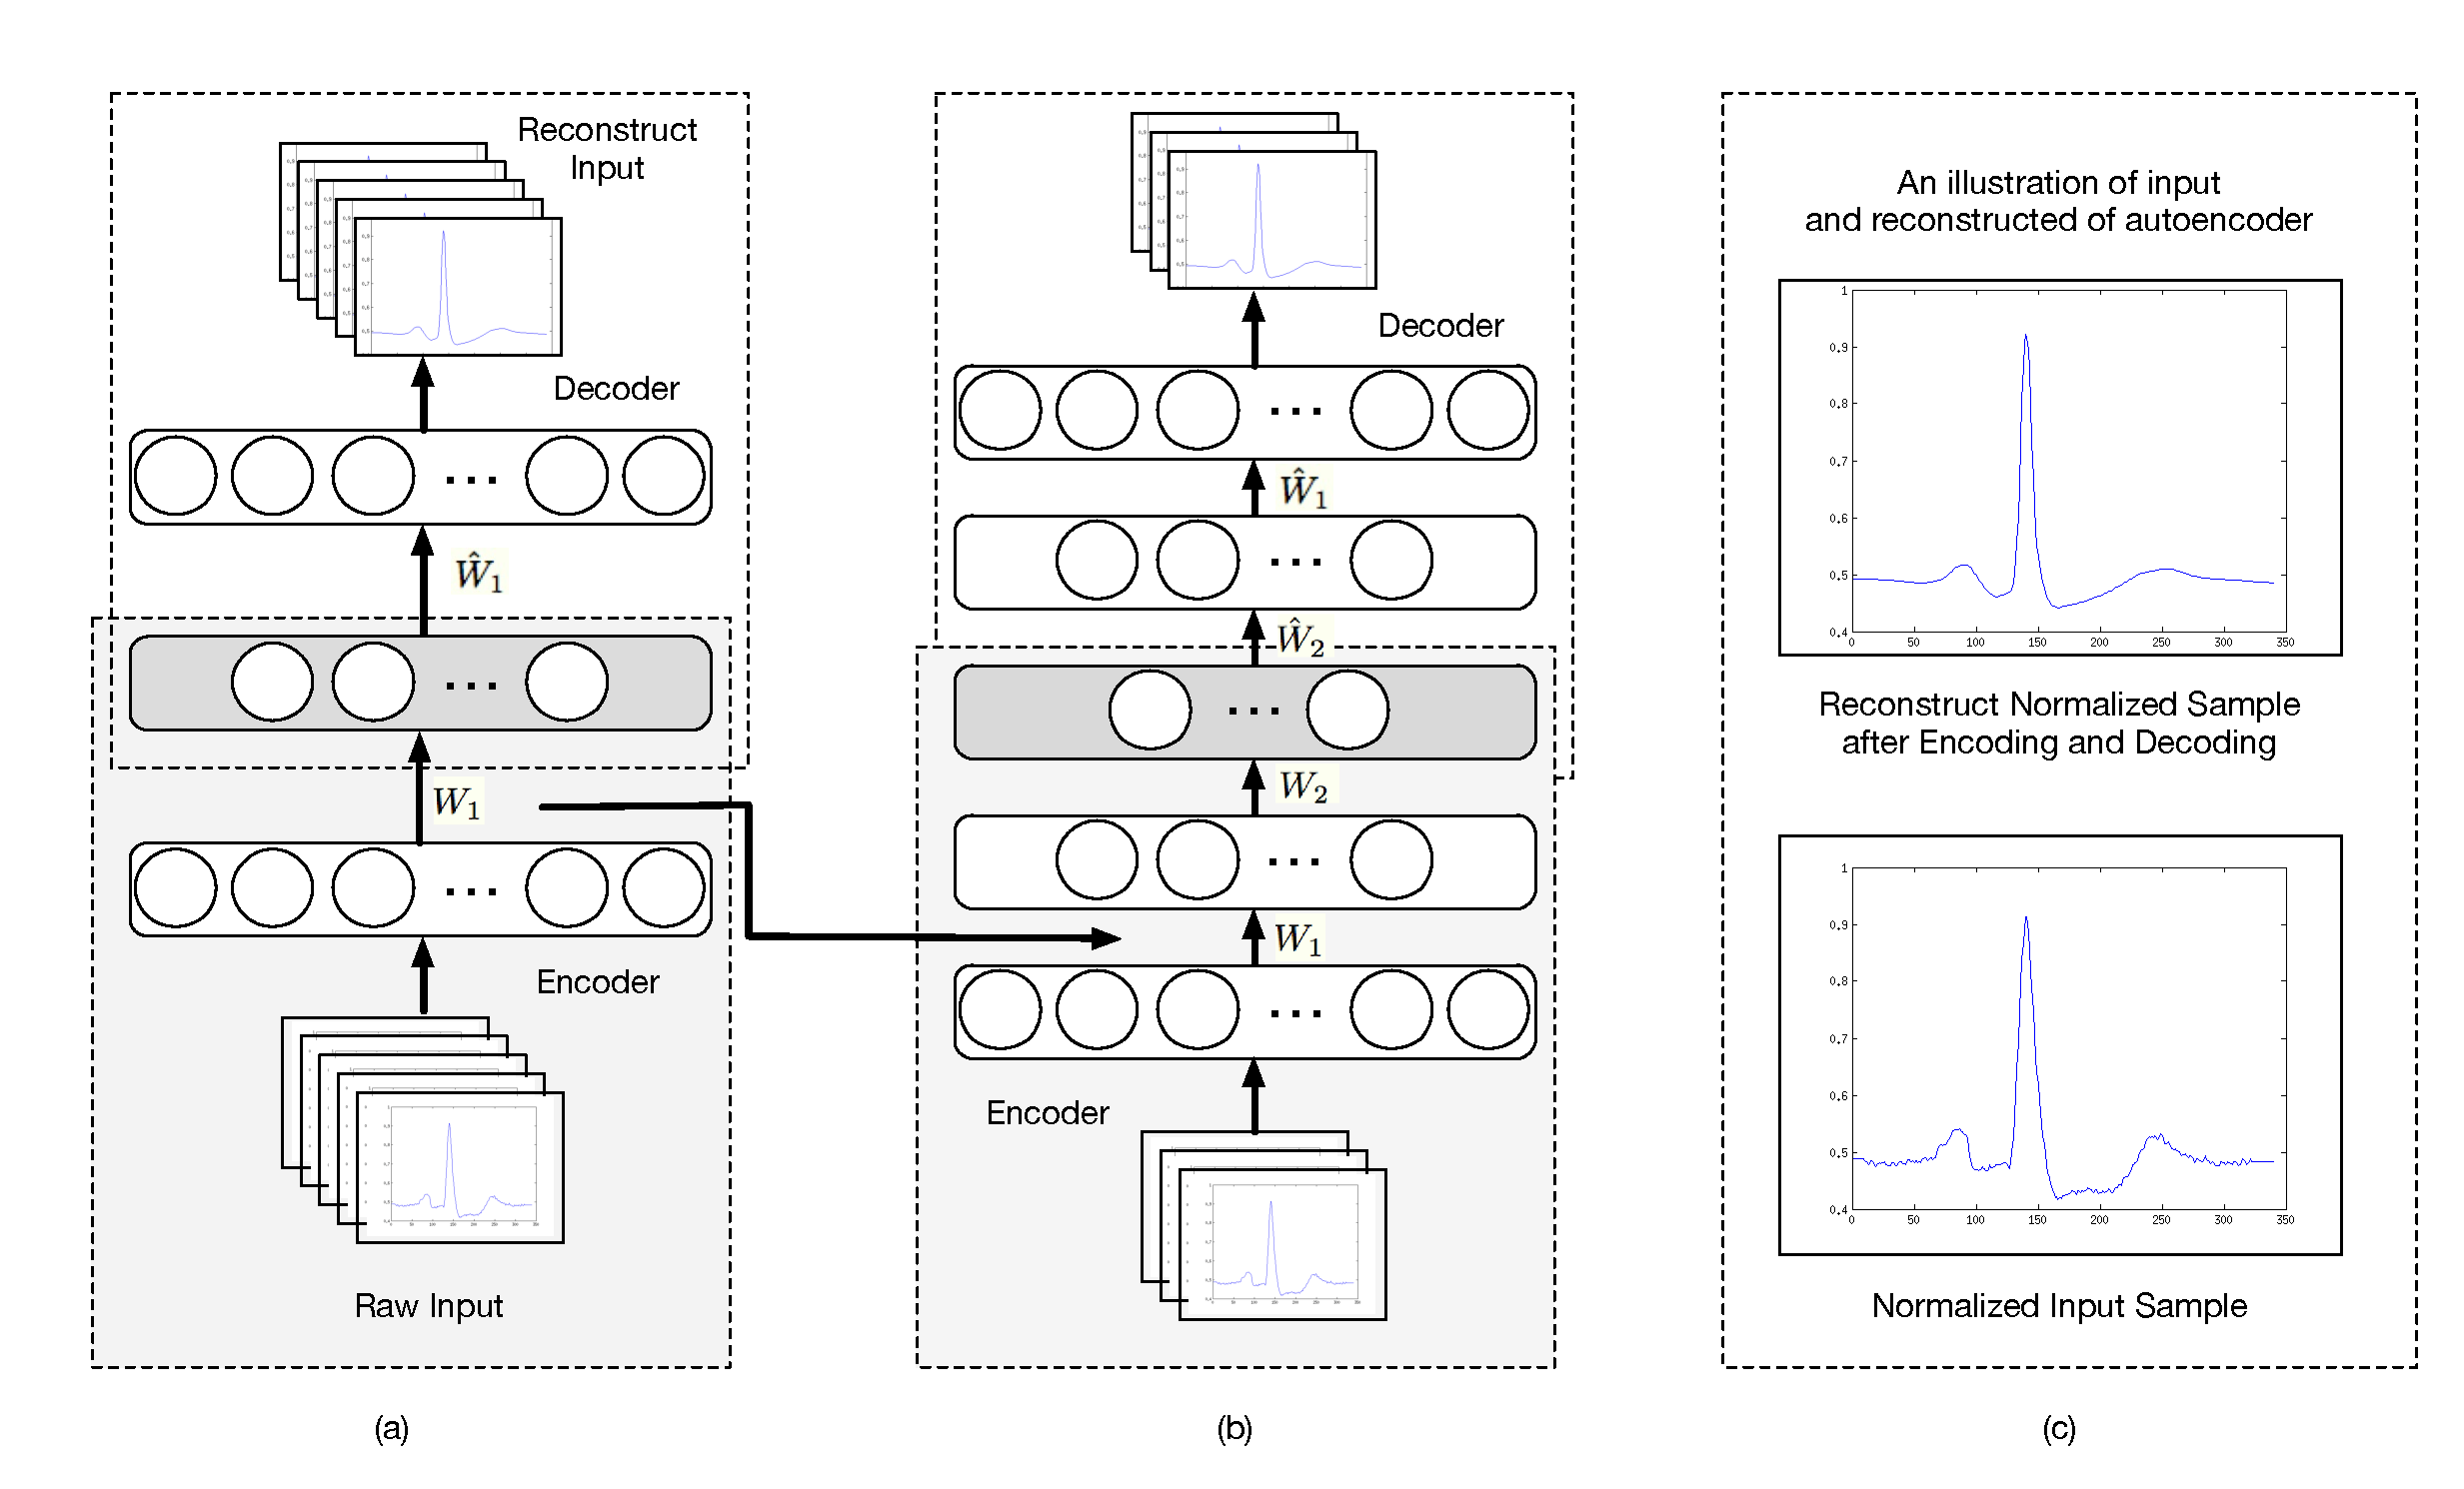
\includegraphics[width=6.5 in]{Figure2}
% where an .eps filename suffix will be assumed under latex, 
% and a .pdf suffix will be assumed for pdflatex; or what has been declared
% via \DeclareGraphicsExtensions.
\caption{The autoencoder pretraining process. (a) of figure 2 illustrated the one-hidden-layer autoencoder encoding and decoding processes; (b) of figure 2 illustrated a deeper network of 2-hidden-layer autoencoder which used the weight $W_1$ and outputs of feature layer (the gray layer) learned in (a); (c) of figure 2 is a comparison of normorlized data of raw input sample and reconstructed sample.}
\label{figure2}
\end{figure*}

The stack autoencoder use multilayer ``encoder" network to transform high dimensional data into low dimensional code, similarly a ``decoder" network can be adopted to recover from the code, which we previously described as a representations or features. For the one-hidden-layer autoencoder input layer and hidden layer as depicted in (a) of Figure \ref{figure2}, as the output was set equal to the input, starting with random weights in the one-hidden layer neural networks, they can be trained together by minimizing the discrepancy between the original input data and its reconstruction. The gradients were obtained by using chain rule of backpropagate error derivatives, the decoder means the raw input can be reconstruct by the learned feature with the trained weight.
With large initial weights, autoencoders typically find poor local minima; with small initial weights, the gradients in the early layers are tiny, making it infeasible to train autoencoders with many hidden layers \cite{hinton}. 

After learning the feature and network weight in the first layer, we can add hidden layer one by one to get deeper representations, as well the learned weight can be used to reconstruct the input. When training the weight of layer 2, we take the weight in layer 1 fixed replace random initialize because the learned weights are close to a good solution, which means training the parameters of each layer individually while freezing parameters for the remainder of the model. The pretraining process is illustrated in Figure \ref{figure2}. As this work focus on the class-action task, so the ``decoding" layers were discarded and link the last hidden layer to the softmax classifier. 



     
     \begin{table}[!htbp]
\begin{center}
\begin{threeparttable}
\caption{Structure Settings}
\label{Table 5}
\begin{tabular}{ccccc}
\hline
&Number of & 2 & 3 &  4\\
&hidden layer& & &\\
\hline
& Nodes & 200$\times$100 & 200$\times$100$\times$100&200$\times$100$\times$100$\times$100 \\

\hline
\end{tabular}
\end{threeparttable}
\end{center}
\end{table}


In the experiment, we adopted 2-hidden-layer, 3-hidden-layer, 4-hidden-layer stacked autoencoder for the test and verify. 

\subsubsection{Fine-tuning}
Fine tuning is a strategy that widely used in deep learning, which can be used to greatly improve the performance of a stacked autoencoder. 
After pretraining multiple layers of feature detectors, the model is ``unfold" to produce encoder and decoder networks that initially use the same weights \cite{hinton}. 
The weights learned can be used for classification implementation after adding one classifier after the feature layer. In this study, a softmax classifier was added (Figure \ref{figure3}). 
In the fine-tuning initialization, the parameters learned in the autoencoder pretraining were used, and the weights $W$ and biases $b$  of softmax classifier (the last layer of the network) were initialized randomly. 
The training set of DS2 were used in the supervised learning pretraining while the backpropagation algorithm as usual of multi-layer perceptrons to minimise the output prediction error has been adopted.

\begin{figure}[]
\centering
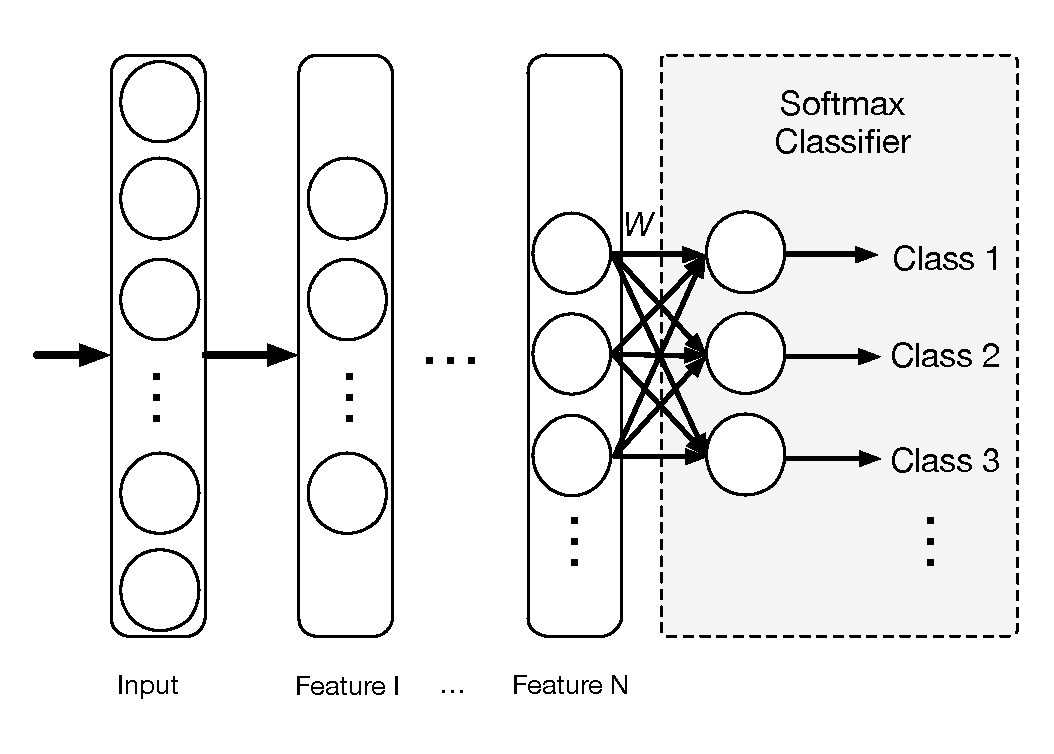
\includegraphics[width=3 in]{Figure3}
% where an .eps filename suffix will be assumed under latex, 
% and a .pdf suffix will be assumed for pdflatex; or what has been declared
% via \DeclareGraphicsExtensions.
\caption{The softmax classifier. In each layer a bias node was included which had not been illustrated in the figure. }
\label{figure3}
\end{figure}

\subsubsection{Test and Classifier Performance Assessment}
After the pretraining and fine-tuning process, the deep network parameters were acquired. Then we use the parameters and the test data set DS3 to predict the class of samples. 
It is necessary to mention that in DS2 and DS3, the labelled data used in pretraining and fine-tuning were divided randomly, which satisfy the requirement of Holdout cross-validation scheme so that the test results were meaningful for the classification task performance improvement.

The following statistical parameters of test performance were used in the study:
\begin{enumerate}
\item Specificity: number of correctly classified normal beats over total number of normal beats.
\item Sensitivity: number of correctly classified abnormal beats over total number of the given abnormal beats.
\item Overall classification accuracy: number of correctly classified beats over number of total beat.
\end{enumerate}


\section{Experimental Results}
\subsection{The Classification Test Results}
As previously mentioned, we adopted three different layer strategies for the classification task. 
In the 2-hidden-layer autoencoder network, we got a accuracy of $99.33\%$. For the N class the specificity is $99.76\%$, the sensitivity of S class is $80.08\%$, the sensitivity of V class is $98.13\%$, the sensitivity of F class is $85.48\%$ as illustrated in Table \ref{table6}. 

\begin{table}[!htbp]
\begin{center}
\begin{threeparttable}
\caption{Test Result for 2-Hidden-Layer Autoencoder Network}
\label{table6}
\begin{tabular}{cccccccc}
\hline
\multicolumn{6}{r}{Algorithm label} \\
\cline{3-7}
&  & N & S & V & F & Q & T\\
\hline
 Reference & N & 41,965 &  39  &  45  & 13  &  6  &  42,068 \\
	label & S &  91   & 398  &  6   & 2   & 0   &  497\\
			      & V &  63   & 3    & 3,940 & 5   & 4   &  4,015\\
			      & F &  23   & 0    & 13   & 212 & 0   &  248\\
			      & Q & 2     & 1    & 0    & 1   & 0   &  3\\
\hline
\end{tabular}
\begin{tablenotes}
\item The test accuracy is about $99.33\%$.
\end{tablenotes}
\end{threeparttable}
\end{center}
\end{table}

In the 3-hidden-layer autoencoder network, we got a accuracy of $99.07\%$. For the N class the specificity is $99.64\%$, the sensitivity of S class is $75.14\%$, the sensitivity of V class is $97.58\%$, the sensitivity of F class is $80.33\%$ as illustrated in Table \ref{table6}. 

\begin{table}[!htbp]
\begin{center}
\begin{threeparttable}
\caption{Test Result for 3-Hidden-Layer Autoencoder Network}
\label{table6}
\begin{tabular}{cccccccc}
\hline
\multicolumn{6}{r}{Algorithm label} \\
\cline{3-7}
&  & N & S & V & F & Q & T\\
\hline
 Reference & N & 41,721 &  66  &  66  & 19  &  0 &  41,872 \\
	label & S &  120  & 405  &  13  & 1   & 0  &  539\\
			   & V &  74   & 10   & 4,073 & 17  & 0  &  4,174\\
			   & F &  27   & 2    & 19   & 196 & 0  &  244\\
			   & Q & 2     & 0    & 0    & 1   & 0  &  2\\
\hline
\end{tabular}
\begin{tablenotes}
\item The test accuracy is about $99.07\%$.
\end{tablenotes}
\end{threeparttable}
\end{center}
\end{table}

In the 4-hidden-layer autoencoder network, we got a accuracy of $99.34\%$. For the N class the specificity is $99.74\%$, the sensitivity of S class is $82.29\%$, the sensitivity of V class is $98.31\%$, the sensitivity of F class is $87.71\%$ as illustrated in Table \ref{table7}. 


\begin{table}[!htbp]
\begin{center}
\begin{threeparttable}
\caption{Test Result for 4-Hidden-Layer Autoencoder Network}
\label{table7}
\begin{tabular}{cccccccc}
\hline
\multicolumn{6}{r}{Algorithm label} \\
\cline{3-7}
&  & N & S & V & F & Q & T\\
\hline
 Reference & N & 41,778 &  38  &  48  & 17  & 5  &  41,886 \\
	label & S &  93   & 460  &   3  & 1   & 2  &  559\\
			   & V &  52   & 1    & 4,067 & 11  & 6  &  4,137\\
			   & F &  15   & 0    & 13   & 214 & 2  &  244\\
			  & Q &  1    & 0    & 1    & 1   & 1  &  5\\
\hline
\end{tabular}
\begin{tablenotes}
\item The test accuracy is about $99.34\%$.
\end{tablenotes}
\end{threeparttable}
\end{center}
\end{table}

\begin{figure}[]
\centering
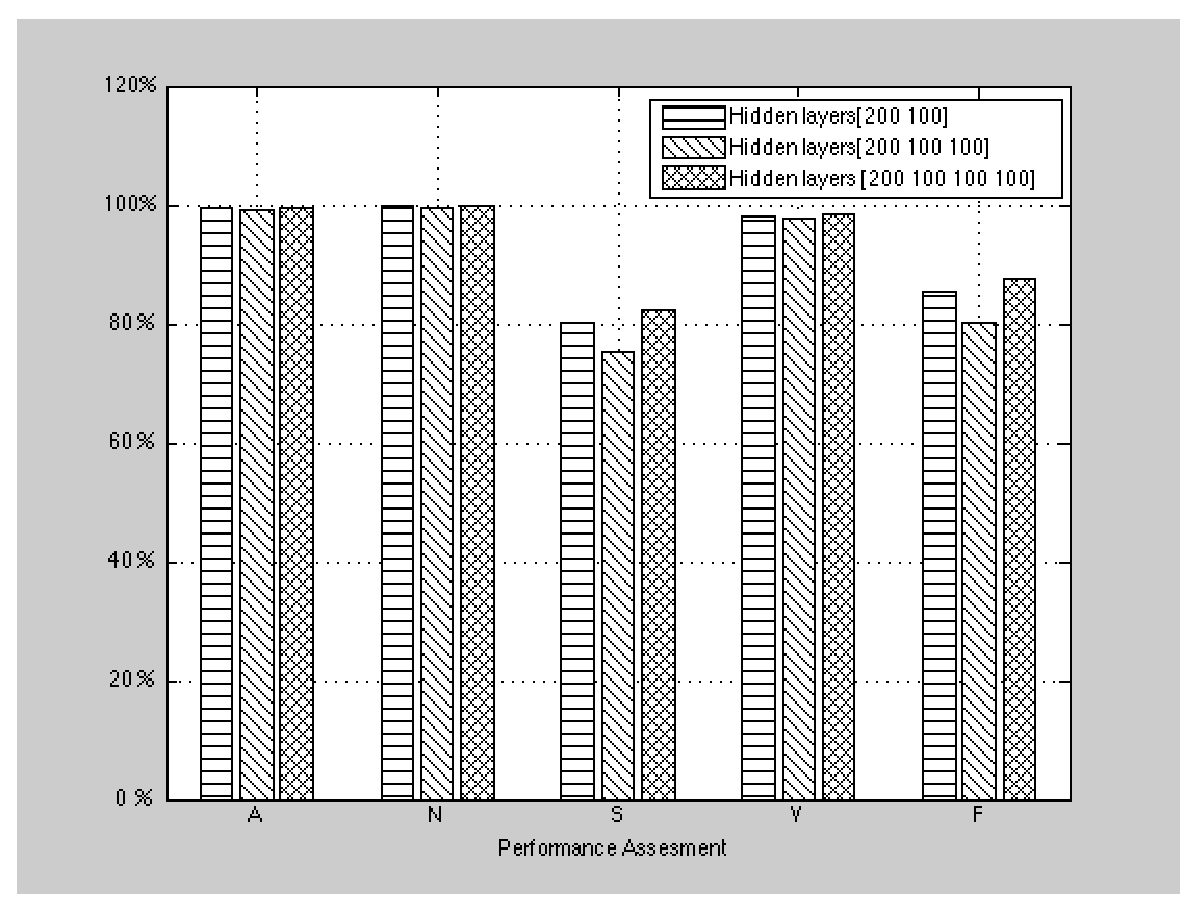
\includegraphics[width=3.2 in]{Figure4}
% where an .eps filename suffix will be assumed under latex, 
% and a .pdf suffix will be assumed for pdflatex; or what has been declared
% via \DeclareGraphicsExtensions.
\caption{The comparison of 3 kinds of network structure.}
\label{figure4}
\end{figure}
As the comparisons in Figure \ref{figure4} illustrated, the general accuracy of our proposed approach for classification task is more than 99\%, the normal heartbeat class specificity is 99.64\%, the supraventricular heartbeat average sensitivity is more than 80\%, the ventricular sensitivity is more than 98\%, and the fusion class sensitivity is about 86\%.

\subsection{Comparisons with Other Work}
In this study, we proposed a Big Data based approach for the heartbeat arrhythmia classification, the arrhythmia classification problem had been discussed in lots of literatures as the reference listed. Different kinds of performance assessment criteria had been adopted. In the comparison part, we adopt several ordinary indicators for the performance assessment, which brought in the above sections. The accuracies, N-class specificities (N-spe), S-class sensitivities (S-sen), V-class sensitivities (V-sen) and the F-class sensitivities(F-sen) in Table \ref{table9} are presented for the comparison. The percentages are calculated from the literatures' test results, in which some of the classes are ignored like \cite{melgan}, we use a $*$ symbol to represent the result are not available. 
In Table \ref{table9}, we use the highest value (2 to 4 hidden layers based structures) for the verification which illustrated in ``proposed" line.

\begin{table}[!htbp]
\begin{center}
\begin{threeparttable}
\caption{Comparisons with Other Work}
\label{table9}
\begin{tabular}{lllllll}
\hline

Approaches&  Accuracy & N-spe & S-sen & V-sen & F-sen \\
\hline
 Proposed & 99.34\% & 99.76\% &  82.29\% & 98.31\% & 87.71\% \\
 Mar\cite{mar} & 84.63\% &84.85\% & 82.90\& & 86.72\% & 51.55\% \\
 Chazal\cite{chaza} &  86.19 \% & 86.86\% & 83.83\% & 77.74\% & 89.43\% \\
 Melgani\cite{melgan} & 90.52\% & 89.12\% & *$^a$& 89.97\% & * \\
 Jiang \cite{jiang} & 94.51\%  &98.73\% & 50.59\% & 86.61\% & 35.78\% \\
\hline
\end{tabular}
\begin{tablenotes}
\item [a] * means the results were not available.
\item [b] The listed percentages are based on the previous described rules.
\end{tablenotes}
\end{threeparttable}
\end{center}
\end{table}

Through the comparisons in Table \ref{table9}, we can see that the proposed method offers better accuracy of classification problem. Since accuracy in lots of the literatures are high enough, the verification parameter depends on mainly on the normal class detection, but on contrary with these methods, this approach provided higher performance in  other arrhythmia waveforms classes. 

\subsection{The Filter Influence for Classification}
\begin{figure}[]
\centering
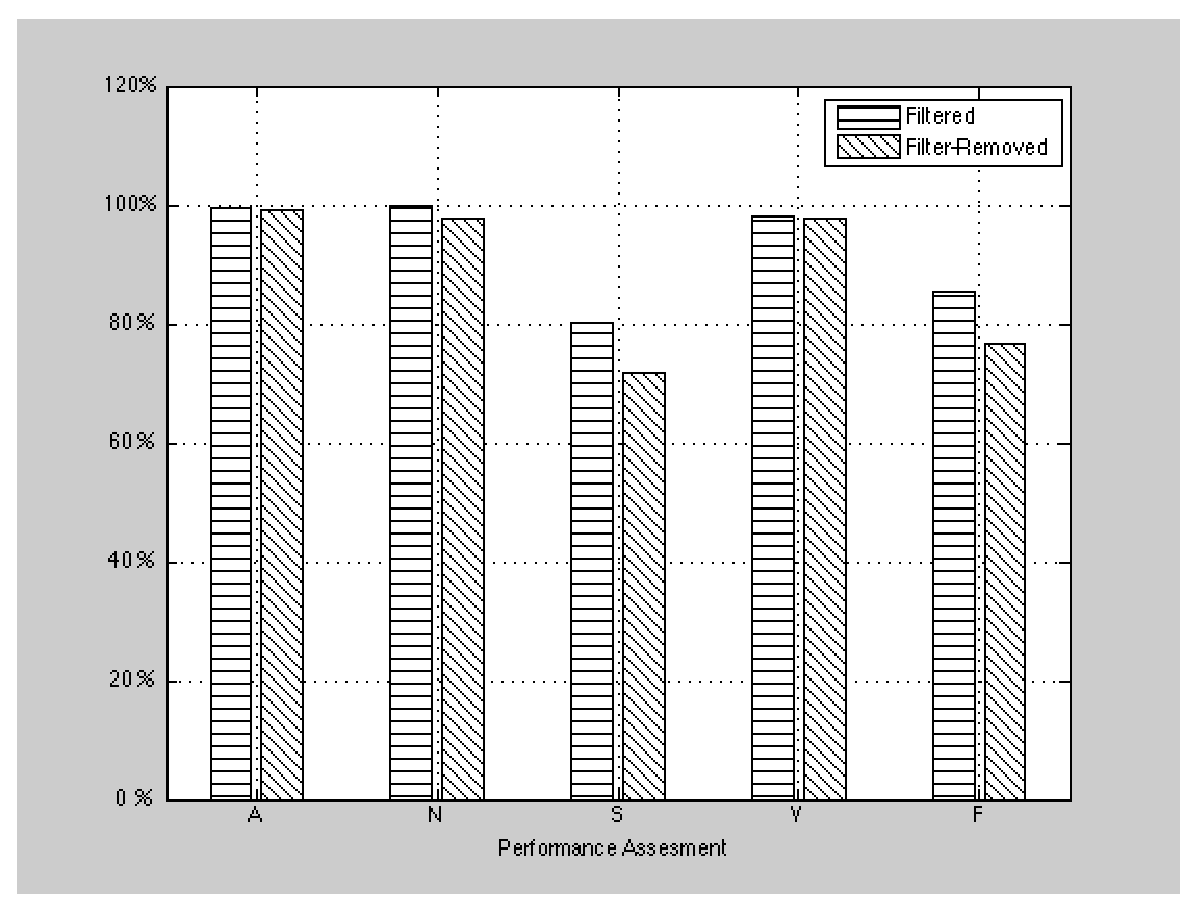
\includegraphics[width=3.2 in]{Figure5}
\caption{The comparisons between filtered and filter-removed performance.}
\label{figure5}
\end{figure}

In the setup section, the proposed preprocessing include the baseline remove process without any further preprocessing. The classification results in Table \ref{table8} illustrate a 2-hidden-layer classification without any filtering procedures. The accuracy of the filter-removed classification is $99.07\%$, for the N class the specificity is $97.58\%$, the sensitivity of S class is $71.89\%$, the sensitivity of V class is $97.77\%$, the sensitivity of F class is $76.82\%$ as illustrated in Table \ref{table8}. The comparison between the two preprocessing procedures is illustrated in Figure \ref{figure5}.

\begin{table}[!htbp]
\begin{center}
\begin{threeparttable}
\caption{Test Result for 2-Hidden-Layer without Filtering}
\label{table8}
\begin{tabular}{cccccccc}
\hline
\multicolumn{6}{r}{Algorithm label} \\
\cline{3-7}
&  & N & S & V & F & Q & T\\
\hline
 Reference & N & 41847 & 54   & 52   & 13  & 0  &  42866 \\
	label & S & 141   & 376  & 6    & 0   & 0  &  523\\
		   & V & 74    & 9    & 3941 & 13  & 0  &  4031\\
			   &F & 51    & 1    & 18   & 232  & 0  &  302\\
			  & Q & 1     & 0    & 1    & 1   & 0  &  3\\
\hline
\end{tabular}
\begin{tablenotes}
\item The test accuracy is about $99.07\%$.
\end{tablenotes}
\end{threeparttable}
\end{center}
\end{table}


As the results comparisons in Figure \ref{figure5}, we find out that the general accuracy, normal heartbeat specificity and ventricular ectopic heartbeat sensitivity have similar performance between the filtered and filter-removed procedures. The supraventricular ectopic beat and fusion beat sensitivity vary slightly. From which we can state that the baseline removal filter affect the classification minor in our proposed approach. The effect of filtering or smoothing for the input signal might be seen in Figure \ref{figure1} part (c) from the autoencoder reconstruction process. The reason would be discussed in the discussion section.


\section{Discussions}

The above results confirm that starting the supervised classification from pre-trained weights of deep networks rather than using random initialised weights would yield better performance.
As the experimental results had been shown, the discussions are going to be presented in this section.
\subsection{The autoencoder feature expression ability and pre training}
If one is going to have fixed-size representations, the sparse representations are more efficient than non-sparse ones in an information-theoretic sense \cite{hinton}. 
Deep learning strategies are based on learning internal representations of data, the learned features or representations from the structure act as roles of the various artificial features adopted in vast literatures. It impossible to explain what the exact features are from the feature layer, but these self-learned representations can be adopted to get good results for our classification task.

Thought adopting unsupervised stacked autoencoder training with a large unlabelled dataset need a prolonged training time, the classification implementation would not be time consuming since we only need to keep the trained weights and bias parameters then a new heartbeat can be categorized. 

\subsection{Test results}
As the figures and tables in the experiment results shows, generally a better classification result had been achieved by the proposed method. Especially for the S and F category, because the sample amount in the datasets (both unlabelled of DS1, and labelled of DS2 and DS3), the sensitivities were not as good performance as the V and N class. 
As the for the better performance than artificial-feature-based classification approaches, we may expect better performances on S and F if more samples were involved.

\subsection{The Filtering Preprocess Impact}
We adopt the same network structure and training method between a pure input experiment and a baseline filter out experiment. The comparison in Figure \ref{figure5} shows that a general accuracy, N specificity and V sensitivity are quite similar, while S and F make a slightly difference. The explain for the effect might be the weakness of the noise representation in the feature layer, the related weights would not affect the classification. In the S and F class comparisons, the difference due to the relatively less training examples, the noise representation affect the classification more.
All the proposed results are based on only baseline wander removed for a better performance for S and F class.
We believe that a better performance would be achieved while more S and F samples added in training.





\section{Conclusions}
Since the deep neural network structure and deep learning algorithms had been widely used in modern computing science especially in Big Data processes, this study proposed one possibility to adopt this method in the health informatics applications. 
In the above content, a stacked autoencoder based algorithm and deep neural network structure are proposed for the arrhythmia classification task.  
The MIT-BIH Arrhythmia Database, MIT Long-Term Database and an unlabelled ambulatory ECG dataset were used in this study to achieve the arrhythmia classification according to the AAMI standard.
We test 46,831 samples randomly chosen from MIT-BIH AR(16,831) and MIT-BIH LT(30,000) and the highest classification accuracy is 99.33\%, for normal heartbeat the specificity attains 99.76\%, for supraventricular ectopic heartbeat the sensitivity reach  82.29\%, for ventricular ectopic heartbeat the sensitivity achieve 98.31\% and 87.71\% for fusion heartbeat.

More than the achieved better performance for classification, we proposed a new possibility to make use of the large amount of unlabelled data from the long-term clinical monitoring and healthcare monitoring. The healthcare data of ECG analysis based on Big Data acquired from wearable devices could be one important occasion for the proposed method.





% You must have at least 2 lines in the paragraph with the drop letter
% (should never be an issue)



% needed in second column of first page if using \IEEEpubid
%\IEEEpubidadjcol


% An example of a floating figure using the graphicx package.
% Note that \label must occur AFTER (or within) \caption.
% For figures, \caption should occur after the \includegraphics.
% Note that IEEEtran v1.7 and later has special internal code that
% is designed to preserve the operation of \label within \caption
% even when the captionsoff option is in effect. However, because
% of issues like this, it may be the safest practice to put all your
% \label just after \caption rather than within \caption{}.
%
% Reminder: the "draftcls" or "draftclsnofoot", not "draft", class
% option should be used if it is desired that the figures are to be
% displayed while in draft mode.
%
%\begin{figure}[!t]
%\centering
%\includegraphics[width=2.5in]{myfigure}
% where an .eps filename suffix will be assumed under latex, 
% and a .pdf suffix will be assumed for pdflatex; or what has been declared
% via \DeclareGraphicsExtensions.
%\caption{Simulation Results.}
%\label{fig_sim}
%\end{figure}

% Note that IEEE typically puts floats only at the top, even when this
% results in a large percentage of a column being occupied by floats.


% An example of a double column floating figure using two subfigures.
% (The subfig.sty package must be loaded for this to work.)
% The subfigure \label commands are set within each subfloat command,
% and the \label for the overall figure must come after \caption.
% \hfil is used as a separator to get equal spacing.
% Watch out that the combined width of all the subfigures on a 
% line do not exceed the text width or a line break will occur.
%
%\begin{figure*}[!t]
%\centering
%\subfloat[Case I]{\includegraphics[width=2.5in]{box}%
%\label{fig_first_case}}
%\hfil
%\subfloat[Case II]{\includegraphics[width=2.5in]{box}%
%\label{fig_second_case}}
%\caption{Simulation results.}
%\label{fig_sim}
%\end{figure*}
%
% Note that often IEEE papers with subfigures do not employ subfigure
% captions (using the optional argument to \subfloat[]), but instead will
% reference/describe all of them (a), (b), etc., within the main caption.


% An example of a floating table. Note that, for IEEE style tables, the 
% \caption command should come BEFORE the table. Table text will default to
% \footnotesize as IEEE normally uses this smaller font for tables.
% The \label must come after \caption as always.
%
%\begin{table}[!t]
%% increase table row spacing, adjust to taste
%\renewcommand{\arraystretch}{1.3}
% if using array.sty, it might be a good idea to tweak the value of
% \extrarowheight as needed to properly center the text within the cells
%\caption{An Example of a Table}
%\label{table_example}
%\centering
%% Some packages, such as MDW tools, offer better commands for making tables
%% than the plain LaTeX2e tabular which is used here.
%\begin{tabular}{|c||c|}
%\hline
%One & Two\\
%\hline
%Three & Four\\
%\hline
%\end{tabular}
%\end{table}

% Note that IEEE does not put floats in the very first column - or typically
% anywhere on the first page for that matter. Also, in-text middle ("here")
% positioning is not used. Most IEEE journals use top floats exclusively.
% Note that, LaTeX2e, unlike IEEE journals, places footnotes above bottom
% floats. This can be corrected via the \fnbelowfloat command of the
% stfloats package.





% if have a single appendix:
%\appendix[Proof of the Zonklar Equations]
% or
%\appendix  % for no appendix heading
% do not use \section anymore after \appendix, only \section*
% is possibly needed

% use appendices with more than one appendix
% then use \section to start each appendix
% you must declare a \section before using any
% \subsection or using \label (\appendices by itself
% starts a section numbered zero.)
%


\appendices
\section{Notations}
\begin{itemize}
\item $x$: Input features for training example, $x \in \Re^{(n+1)}$.
\item $y$: Output values, in the case of the autoencoder, $y=x$.
\item $(x^{(i)},y^{(i)})$: the $i$-th training example.
\item $W_{(ij)}^{(l)}$: The parameter of the connection between unit $j$ in layer $l$, and unit $i$ in layer $l+1$.
\item $b_i^{(l)}$: The bias term associated with unit $i$ in layer $l+1$.
\item $\theta$: Parameter vector taking $W$ and $b$.
\item $a_i^{(l)}$: Activation (output) of unit $i$ in layer $l$ of the network while layer $l_1$ is the input layer, we also have $a^{(1)}_i = x_i$.
\item $f(\cdot)$: The activation function, a $sigmoid$ function were used in this study: $f(z) = sigmoid(z)$.
\item $z_i^{(l)}$: Total weighted sum of inputs to unit $i$ in layer $l$.
\item $\alpha$: Learning rate parameter.
\item $s_l$: Number of units in layer $l$ (without the bias unit).
\item $n_l$: Number of layers.
\item $\lambda$: Weight decay parameter.
\item $\hat{x}$: Output of autoencoder, the reconstruction of $x$, the same as $h_{W,b}(x)$.
\item $\rho$: Sparsity parameter
\item $\hat{\rho}_i$: The average activation of hidden unit $i$ (in autoencoder).
\item $\beta$: Weight of sparsity penalty term.

\end{itemize}
% you can choose not to have a title for an appendix
% if you want by leaving the argument blank


% use section* for acknowledgement
\section*{Acknowledgment}
This study was financed partially by the National 863 Program of China (Grant No. 2012AA02A604), the Next generation communication technology Major project of National S\&T (Grant No. 2013ZX03005013), the Key Research Program of the Chinese Academy of Sciences, and the Guangdong Innovation Research Team Funds for Image-Guided Therapy and Low-cost Healthcare. 
% Can use something like this to put references on a page
% by themselves when using endfloat and the captionsoff option.
\ifCLASSOPTIONcaptionsoff
  \newpage
\fi



% trigger a \newpage just before the given reference
% number - used to balance the columns on the last page
% adjust value as needed - may need to be readjusted if
% the document is modified later
%\IEEEtriggeratref{8}
% The "triggered" command can be changed if desired:
%\IEEEtriggercmd{\enlargethispage{-5in}}

% references section

% can use a bibliography generated by BibTeX as a .bbl file
% BibTeX documentation can be easily obtained at:
% http://www.ctan.org/tex-archive/biblio/bibtex/contrib/doc/
% The IEEEtran BibTeX style support page is at:
% http://www.michaelshell.org/tex/ieeetran/bibtex/
%\bibliographystyle{IEEEtran}
% argument is your BibTeX string definitions and bibliography database(s)
%\bibliography{IEEEabrv,../bib/paper}
%
\bibliographystyle{IEEEtran} % Style BST file
\bibliography{bare_jrnl}  
% <OR> manually copy in the resultant .bbl file
% set second argument of \begin to the number of references
% (used to reserve space for the reference number labels box)
%\begin{thebibliography}{2}

%\bibitem{tanis}
%T.~Mar, S.~Zaunseder, J.P.~Martinez, M.~Llamedo and R.~Poll, \emph{Optimization of electrocardiography Classification by Means of Feature Selection}.\hskip 1em plus
%  0.5em minus 0.4em\relax Harlow, England: Addison-Wesley, 1999.
  
%\bibitem{care}
%H.~Kopka and P.~W. Daly, \emph{A Guide to \LaTeX}, 3rd~ed.\hskip 1em plus
%  0.5em minus 0.4em\relax Harlow, England: Addison-Wesley, 1999.
  
%\end{thebibliography}

% biography section
% 
% If you have an EPS/PDF photo (graphicx package needed) extra braces are
% needed around the contents of the optional argument to biography to prevent
% the LaTeX parser from getting confused when it sees the complicated
% \includegraphics command within an optional argument. (You could create
% your own custom macro containing the \includegraphics command to make things
% simpler here.)
%\begin{IEEEbiography}[{\includegraphics[width=1in,height=1.25in,clip,keepaspectratio]{mshell}}]{Michael Shell}
% or if you just want to reserve a space for a photo:

\begin{IEEEbiography}{Jan Doe}
Biography text here.
\end{IEEEbiography}
% if you will not have a photo at all:
\begin{IEEEbiographynophoto}{John Doe}
Biography text here.
\end{IEEEbiographynophoto}

% insert where needed to balance the two columns on the last page with
% biographies
%\newpage

\begin{IEEEbiographynophoto}{Jane Doe}
Biography text here.
\end{IEEEbiographynophoto}

% You can push biographies down or up by placing
% a \vfill before or after them. The appropriate
% use of \vfill depends on what kind of text is
% on the last page and whether or not the columns
% are being equalized.

%\vfill

% Can be used to pull up biographies so that the bottom of the last one
% is flush with the other column.
%\enlargethispage{-5in}



% that's all folks
\end{document}


